\documentclass[a4paper, 12pt, final, garamond]{book}
%\usepackage{cours-preambule}
\usepackage{bpep_full}

\raggedbottom

\makeatletter
\renewcommand{\@chapapp}{\'Electrocin\'etique -- chapitre 3}
\makeatother

\begin{document}
\setcounter{chapter}{2}

\newcommand{\f}[2]{{
		\mathchoice
		{\dfrac{#1}{#2}}
		{\dfrac{#1}{#2}}
		{\frac{#1}{#2}}
		{\frac{#1}{#2}}
}}
\newcommand{\e}[1]{{}_{\text{#1}}}

\toggletrue{corrige}  % décommenter pour passer en mode corrigé

\resetQ
\chapter{\sujetUniquement{TD~: capacit\'es et inductances}\siCorrige{Correction du TD}}

\section{Quelle courbe pour quel circuit~?}

\resetQ
\begin{minipage}{0.46\linewidth}
    Um étudiantx distrait, mais surtout maladroitx, rentrant d’une séance de
    travaux pratiques sur l'observation de régimes transitoires sur les circuits
    du premier ordre, fait tomber toutes ses notes qui s’éparpillent. En les
    rangeant, iel retrouve alors 2 courbes expérimentales, tracées en utilisant
    une résistance $R = \SI{1}{k\Omega}$, mais iel ne sait plus à quel montage
    les attribuer.
\end{minipage}
\hfill
\begin{minipage}{0.45\linewidth}
    \begin{center}
        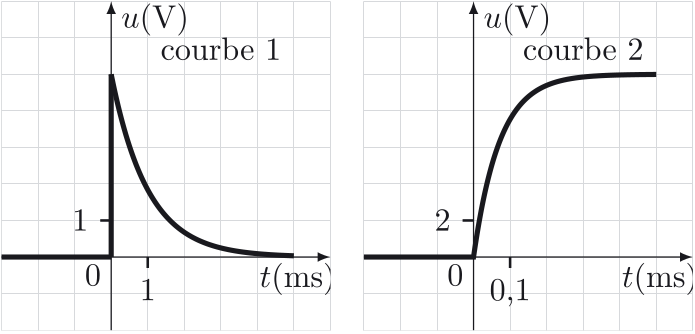
\includegraphics[width=\linewidth]{quellecourbe}
    \end{center}
\end{minipage}

\begin{center}
    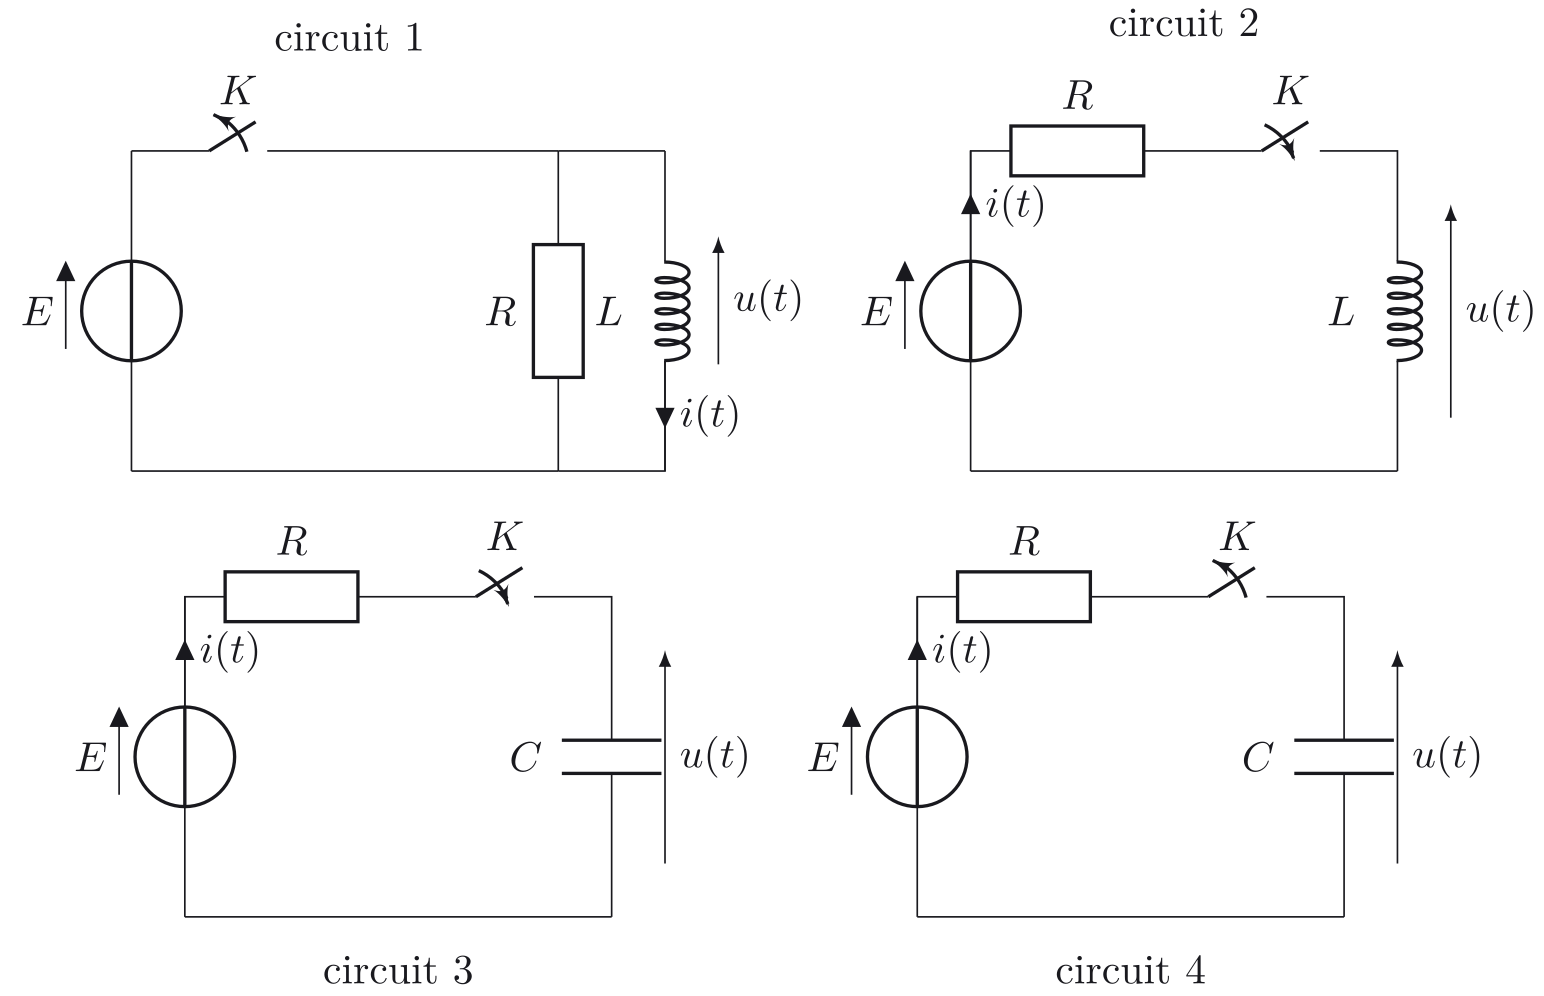
\includegraphics[width=.7\linewidth]{quelcircuit}
\end{center}

\QR{Associer chaque courbe avec l'un des 4 montages ci-dessus, et calculer les
    valeurs de $E$ et $L$ ou $C$ utilisées. Tous les interrupteurs s’ouvrent ou
se ferment à $t = 0$.}{
    \begin{itemize}
        \item Pour la courbe 1~: on observe une diminution exponentielle de la
            \textbf{tension} et une \textbf{discontinuité} de cette dernière en
            $t=0$. Or, les condensateurs ont une tension continue à leurs
            bornes, cette courbe ne peut donc \textbf{pas} être issue d'un
            circuit avec un \textbf{condensateur}~: ni le 3, ni le 4.\bigbreak

            Ensuite, comme c'est forcément une bobine, on observe que $u = L
            \dv{i}{t} > 0$, autrement dit l'intensité monte dans le circuit. Le
            circuit 1 s'ouvre à $t=0$, donc l'intensité devrait y baisser~:
            finalement il ne nous reste que le \textbf{circuit 2}.\bigbreak

            Dans ce circuit, la constante de temps est connue (cf.\ cours) et
            vaut $\tau = L/R$. On la détermine avec l'intersection entre la
            tangente en $t=0$ et l'asymptote $u=0$, où en trouvant l'instant où
            $u$ et son asymptote ont un écart relatif de 37\%, c'est-à-dire ici
            quand $u(\tau) = \SI{1.8}{V}$. On trouve dans tous les cas
            \fbox{$\tau = \SI{1.0}{ms}$}, soit \fbox{$L = \SI{1.0}{H}$}.
        \item Pour la courbe 2~: on observe une augmentation exponentielle de la
            tension et un continuité de cette dernière en $t=0$. On peut donc
            affirmer que $u$ est la tension aux bornes d'un ondensateur, et que
            ce dernier se charge~: on y associe donc le \textbf{circuit
            3}.\bigbreak
            L'asymptote quand $t \rightarrow \infty$ est $u = E$, puisqu'alors
            $i=0$ (comportement condensateur RP) et donc toute la tension du
            générateur se retrouve aux bornes de $C$ (et pas de $R$ car $i=0$)~;
            ainsi, \fbox{$E = \SI{10}{V}$}, et $u(\tau) = \SI{6.3}{V}$ ou la
            tangente en 0 donnent \fbox{$\tau = \SI{0.070}{ms}$}~; comme ici
            $\tau = RC$, on trouve \fbox{$C = \SI{7.0e-8}{F}$}.
    \end{itemize}
}

\resetQ
\section{Associations en parallèle}
\subsection{Condensateurs}
\sujetUniquement{\begin{minipage}{0.40\linewidth}
    \begin{center}
        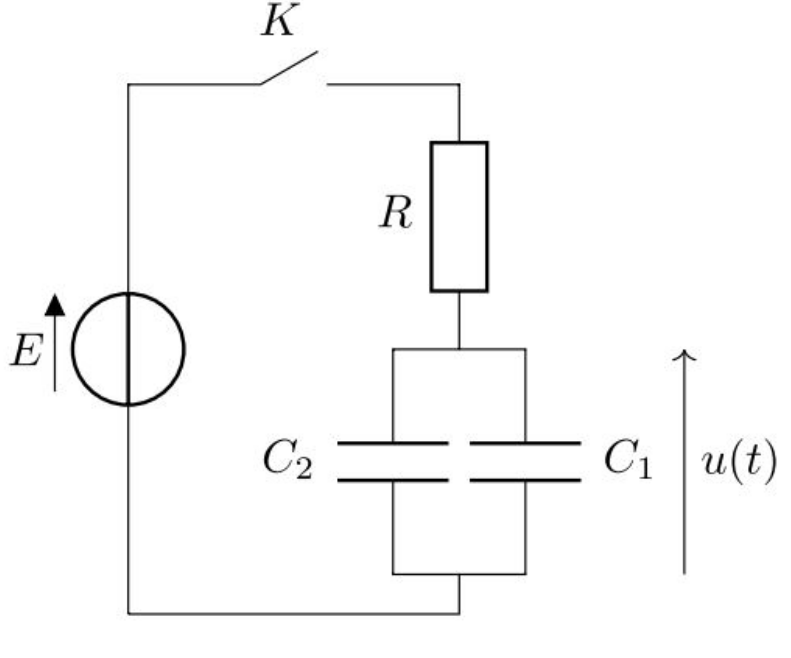
\includegraphics[width=\linewidth]{asso_parr-c}
    \end{center}
\end{minipage}}
\hfill
\begin{minipage}{\sujetUniquement{0.55}\siCorrige{1}\linewidth}
    On considère le circuit ci-contre avec deux condensateurs différents
    associés en parallèle. À $t=0$, les deux condensateurs sont totalement
    déchargés et on ferme l'interrupteur $K$.
    \QR{Déterminer l'équation différentielle satisfaite par $u_(t)$.}{
        Loi des mailles et loi d'Ohm~:
        \[E = u_R + u = Ri + u\]
        Loi des nœuds~:
        \begin{align*}
            i                 & = i_1 + i_2\\
            \Leftrightarrow i & = C_1 \dv{u}{t} + C_2 \dv{u}{t}\\
            \Leftrightarrow i & = (C_1 + C_2) \dv{u}{t}
        \end{align*}
        Ainsi,
        \[\boxed{E = R(C_1+C_2) \dv{u}{t} + u}\]
    }
    \QR{Trouver un composant équivalent aux deux condensateurs en
    parallèle.}{
        On constate qu'électriquement, l'association en parallèle donne un
        condensateur équivalent de capacité \fbox{$C_{\rm eq} = C_1 + C_2$}.
    }
\end{minipage}

\subsection{Bobines}
\sujetUniquement{\begin{minipage}{0.40\linewidth}
    \begin{center}
        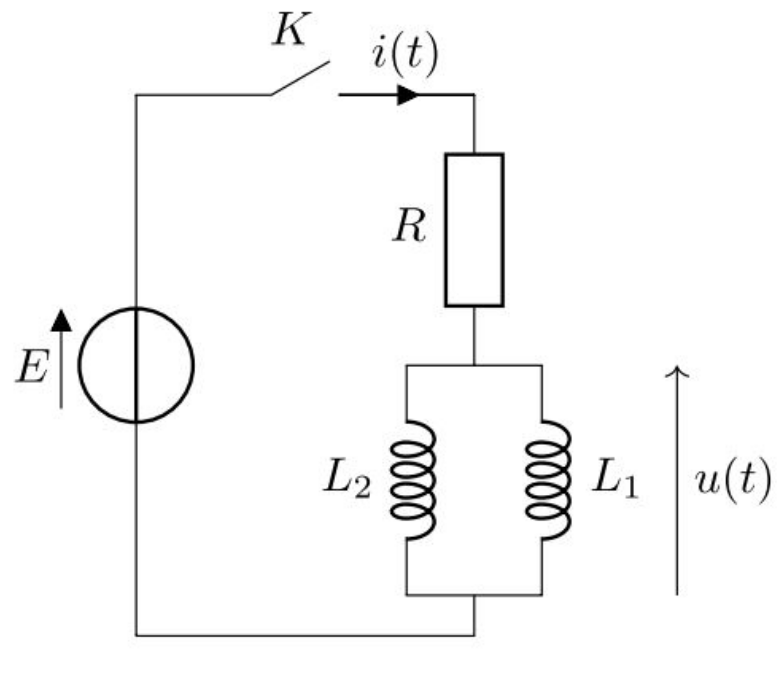
\includegraphics[width=\linewidth]{asso_parr-l}
    \end{center}
\end{minipage}}
\hfill
\begin{minipage}{\sujetUniquement{0.55}\siCorrige{1}\linewidth}
    On considère le circuit ci-contre avec deux bobines différentes
    associées en parallèle. À $t=0$, on ferme l'interrupteur $K$.
    \QR{Déterminer l'équation différentielle satisfaite par $u(t)$.}{
        Loi des mailles et loi d'Ohm~:
        \[E = u_R + u = Ri + u\]
        En dérivant~:
        \[0 = R \dv{i}{t} + \dv{u}{t}\]
        Loi des nœuds~:
        \begin{align*}
            i                     & = i_1 + i_2\\
            \Rightarrow \dv{i}{t} & = \dv{i_1}{t} + \dv{i_2}{t}\\
            \Leftrightarrow \dv{i}{t} & = \frac{u}{L_1} + \frac{u}{L_2}
        \end{align*}
        Ainsi,
        \[\boxed{0 = R\left(\frac{1}{L_1}+ \frac{1}{L_2}\right)u + \dv{u}{t}}\]
    }
    \QR{Trouver un composant équivalent aux deux condensateurs en
    parallèle.}{
        On constate qu'électriquement, l'association en parallèle donne une
        bobine équivalente d'inductance \fbox{$\frac{1}{L_{\rm eq}} =
    \frac{1}{L_1} + \frac{1}{L_2}$}.}
\end{minipage}


\resetQ
\section{Résistance de fuite d'un condensateur}

\begin{minipage}{0.5\linewidth}

    Un condensateur non idéal peut être modélisé par une capacité $C$ associée
    en parallèle avec une résistance $R_f$ appelée résistance de fuite. Ce
    condensateur est complètement chargé sous une tension $E > 0$. Une fois le
    régime permanent atteint, la mesure, à l'aide d’un voltmètre parfait
    (résistance d’entrée infinie), de la tension $u$ aux bornes du condensateur
    est égale à $E$.
\end{minipage}
\hfill
\begin{minipage}{0.45\linewidth}
    \begin{center}
        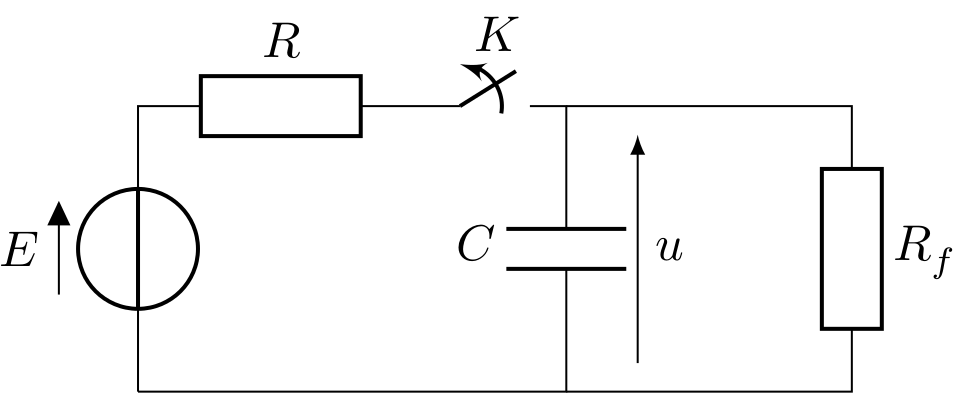
\includegraphics[width=\linewidth]{condo_fuite-plain}
    \end{center}
\end{minipage}

A $t = 0$, on ouvre le circuit. Au bout d’un temps $T > 0$, la valeur mesurée de
$u$ est $E' < E$.

\QR{Comment peut-on expliquer ces observations~?}{ En ouvrant le circuit, sans
    la résistance de fuite on s'attend à ce que le condensateur reste chargé,
    comme une pille. Or dans ce circuit, en ouvrant l'interrupteur la capacité
    $C$ est reliée à la résistance $R_f$ dans laquelle elle se décharge donc, ce
qui explique la diminution de la tension.}

\QR{Donner l'expression de $R_f$ en fonction de $C$, $E$, $E'$ et $T$. Faire
    l'application numérique pour $C = \SI{100}{pF}$, $T = \SI{2}{min}$, $E =
\SI{10}{V}$ et $E' = \SI{1}{V}$.}{
    On a la situation de décharge du cours, où l'équation différentielle sur $u$ est
    \[ \dv{u_C}{t} + \frac{u_C}{R_f C} = 0\]
    Sachant que $u_C(t=0) = E$, la solution s'écrit
    \[\boxed{u_C(t) = E\exp \left( - \frac{t}{R_fC} \right)}\]
    Pour que $u_C(T) = E'$, il faut donc $\exp \left( - \frac{T}{R_fC} \right) =
    \frac{E'}{E}$, et finalement
    \[\boxed{R_f = \frac{T}{C\ln \frac{E}{E'}}} \qqdonc \boxed{R_f \approx
\SI{5.0e11}{\Omega}}\]}

\resetQ
\subimport{/home/nicolas/Documents/Enseignement/Prepa/bpep/exercices/TD/RL_oscilloscope/}{sujet.tex}

\resetQ
\subimport{/home/nicolas/Documents/Enseignement/Prepa/bpep/exercices/TD/regime_transitoire_RC/}{sujet.tex}

\resetQ
\section{Circuit RC à 2 mailles}
\begin{minipage}{0.50\linewidth}
    On considère le circuit représenté ci-contre, dans lequel l'interrupteur $K$
    est fermé à $t=0$.
    \QR{Trouver l'expression de la tension $u(t)$ et tracer son allure.}{
    LdMailles~:
    \[E = Ri + u \qet u_C = u\]
    LdN~:
    \[i = i_1 + i_2 = C \dv{u_C}{t} + \frac{u}{R}\]
    D'où
    \begin{align*}
        E &= RC \dv{u_C}{t} + 2u\\
        \Leftrightarrow \dv{u_C}{t} + \frac{1}{\tau}u + \frac{E}{2\tau}
    \end{align*}
    avec $\tau = \frac{RC}{2}$.\smallbreak
    Après résolution avec $u(0^+) = E$, on obtient
    \[ \boxed{u(t) = \frac{E}{2}(1+e^{-t/\tau})}\]
    Ainsi, $u_C$ décroit exponentiellement de $E$ à $E/2$.
    }
\end{minipage}
\hfill
\begin{minipage}{0.45\linewidth}
    \begin{center}
        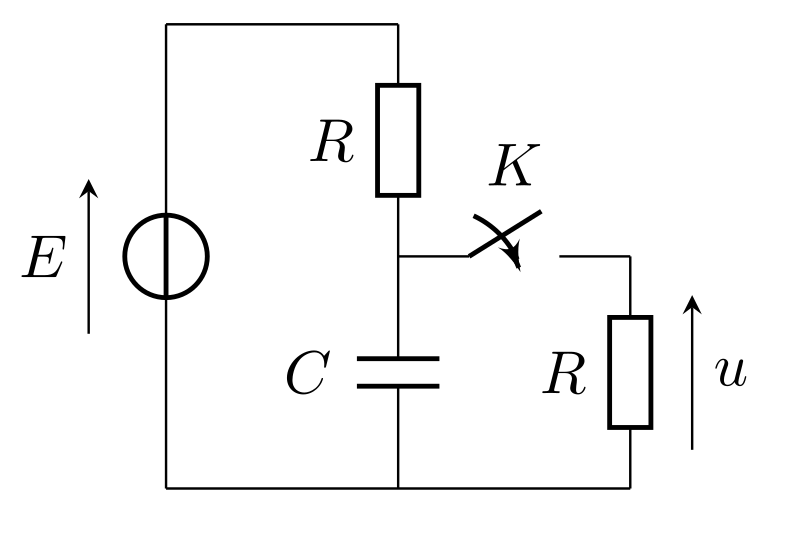
\includegraphics[width=\linewidth]{rc_2mailles-plain}
    \end{center}
\end{minipage}

\resetQ
\subimport{/home/nicolas/Documents/Enseignement/Prepa/bpep/exercices/TD/circuit_RL_RC/}{sujet.tex}

\resetQ
\subimport{/home/nicolas/Documents/Enseignement/Prepa/bpep/exercices/Colle/loi_kirchhoff_3/}{sujet.tex}

\end{document}
